\chapter{FUTURE IMPROVEMENT}

The buffer was designed as a linear buffer that can only provide the offset in the direction that is perpendicular to the direction in which the tractor is moving. However, the tractor cannot move left or right, it can only turn left or right. Therefore, after the sliding occurs, the tractor has to turn to make the correction. In other words, there are some small angles between the planned direction and the actual direction while tractor is moving. In order to cancel these angles, this design needs some improvements.

\section{Improvement to the Buffer}
\begin{figure}[ht!]
\begin{center}
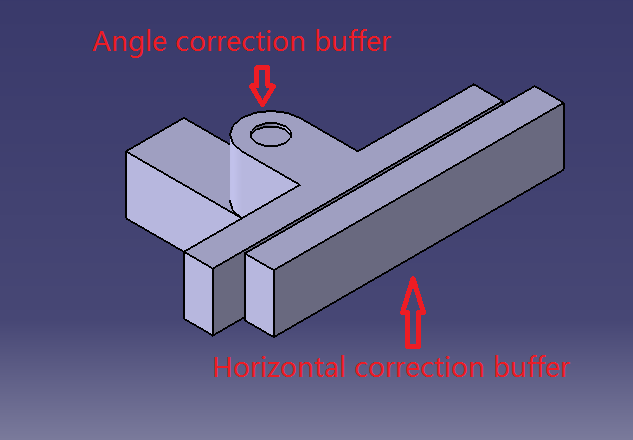
\includegraphics[scale = 0.8]{pics/improvedbuffer.png}
\caption{Improved Buffer}
\end{center}
\end{figure}
Based on the previous design, one more stepper motor needs to be installed, as Figure 7.1 shows, to provide the offset for the angle. The purpose of the stepper motor is to provide a vertical spin to correct the angle error while that tractor is turning. 

\section{Improvement to the Curtain}
\begin{figure}[ht!]
\begin{center}
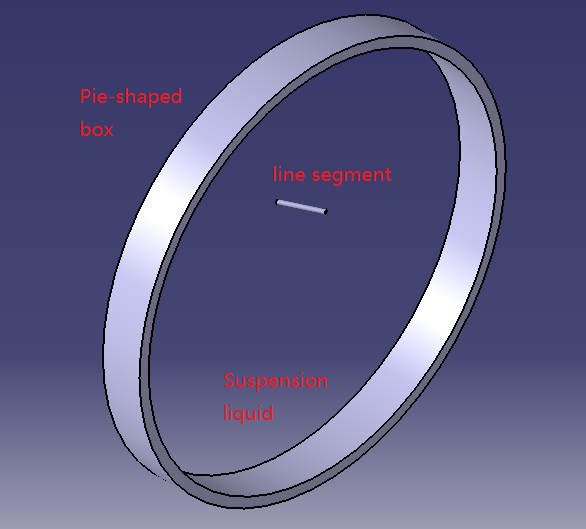
\includegraphics[scale = 0.8]{pics/improvedcurtain.png}
\caption{Improved Curtain}
\end{center}
\end{figure}
Previously, it was introduced that the curtain works like a projection screen. The only trace that the laser left is a spot. Under this situation, it is impossible to find the error angle just from one single spot. The new design for the curtain is a pie-shaped transparent plastic box filled with suspension liquid. Under the semi-transparent environment, the trace of the laser is no longer a spot, but a segment. (Figure 3.8) A segment provides more information than a single spot, and it is easier to find the angle with the direction and length of the segment.

\section{Improvement to the Algorithm}
Base on the developed color detection algorithm, the image captured by the camera shows a line segment. (Figure 3.9)
\begin{figure}[ht!]
\begin{center}
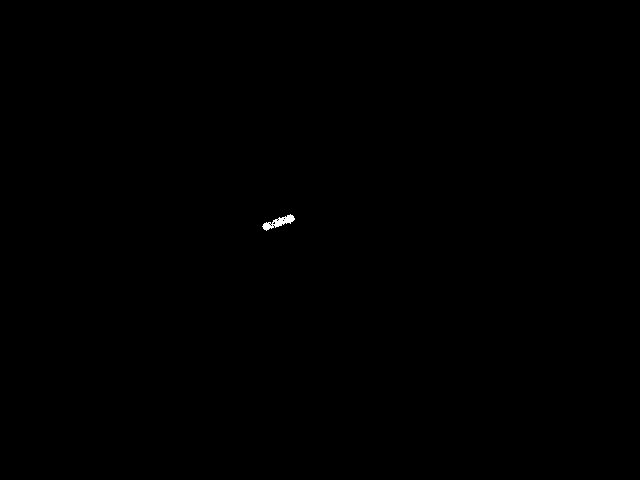
\includegraphics[scale = 0.6]{pics/segment.png}
\caption{Line Segment}
\end{center}
\end{figure}
The improved algorithm finds the angle by the following process. 
\subsection{Coordinates for Each End}

The camera is monitoring the curtain slightly upward, so according to the perspective rule, the upper right end of the segment is the front. For example, the coordinate of upper right end is $(292,217)$, and the coordinate for the lower left end is $(265, 227)$ in Figure 3.9.

\subsection{Projection Length of Segment}

With the coordinates of these two end points, the projection length can be calculated as below, and the unit is pixel. 
\begin{equation}
L = \sqrt{(292-265)^2+(217-227)^2} = 29 \quad pixels
\end{equation}

\subsection{Thickness of the Curtain}

Since the position and the size of the curtain are both fixed, thickness is a constant in this algorithm. This constant was found by taking a picture with the same distance and measuring the pixels on the picture. The thickness of the curtain is 56 $pixels$.

\subsection{Error Angle}

Since the projection length of the segment and the thickness of the curtain are known from the above calculations, the error angle can be calculated with trigonometric function according to the following:
\begin{equation}
Error Angle = tan^{-1}(\frac{29}{56}) = 27.38^o
\end{equation}

According to the perspective rule, the buffer was turned to the right 14.84 degrees. Therefore, this error angle can be corrected by turning the second stepper motor to the left 14.84 degrees. 